\documentclass[11pt]{article}

\usepackage{hyperref}
\usepackage{graphicx}
\usepackage[disable]{todonotes}
%\usepackage{todonotes}
%\usepackage{endnotes}

\usepackage{footnotebackref}



%approximately proportional to symbol
\newcommand{\approptoinn}[2]{\mathrel{\vcenter{
  \offinterlineskip\halign{\hfil$##$\cr
    #1\propto\cr\noalign{\kern2pt}#1\sim\cr\noalign{\kern-2pt}}}}}

\newcommand{\appropto}{\mathpalette\approptoinn\relax}

\title{The Demographics of Taxicab Riders}
\author{Thomas C. Proctor}
\date{}

%\let\footnote=\endnote

\renewcommand{\abstractname}{Executive Summary}
\newcommand{\fref}[1]{Figure~\ref{fig:#1}}
\newcommand{\prsq}{$\mbox{pseudo-}R^2$}

\begin{document}

\maketitle{}

  




In 1937, in response to traffic congestion, New York City began regulating for-hire cars by limiting the total number of vehicles (yellow cabs) that can legally pick up passengers hailed from the street. This has created a system which many say is unfair to those who do not live within the core business district, as accepted wisdom says that unmet demand is high enough within the core business district that there is no incentive for drivers to leave it.
Recently, the advent of other for-hire vehicles in NYC has brought further attention to issues with yellow cabs service across geographic, income, and ethnic groups.
The city has started a system of so called ``boro cabs'', which are allowed to pick up street hails only outside of a defined central business district.
Smartphone hailing apps manage to bypass the regulation scheme based upon street hails, providing significant competition to yellow cabs, along with claims that they better serve poorer neighborhoods.
Along with the conventional wisdom about the locations where cabs can be hailed, there are also other common tropes about cab coverage, such as a bias against non-white passengers and that they are only used by the rich. 
In order to answer any of these questions, we first have to understand the basic demographics of taxicab riders.
%\todo{Re-write Intro to more directly ask the question I answer.}

According to my analysis, the most important factor governing taxi-cab usage is income. More specifically, I find that the number of taxicab drop-offs in a given area per-capita is proportional to the square of the per-capita income in that area.

%\todo{Paragraph about data.}
To understand taxicab usage in NYC, I took a look at the data released by the NYC Taxi and Livery Cab Commission detailing all the roughly 150 million  metered taxi trip taken by licensed NYC cabs, commonly known as yellow cabs.
This data includes longitude and latitude points for the drop-off and pickup locations of each trip.
I compare the drop-offs to demographic data on residents from the U.S Census Bureau that is split up by census tract, which in NYC usually encompasses just a few blocks. 
I counted the number of drop-offs in each census tract so that I could compare the number of drop-offs to the demographic data from the census.

The map below shows New York City, with darker areas indicating a higher number of total drop-offs during 2013 and lighter lower.
The darkest area of the map is the central business district of NYC, midtown Manhattan, with the two airports showing up as the black spots to the right of Manhattan.

%\begin{figure}[h]
%  \centering
\begin{centering}
  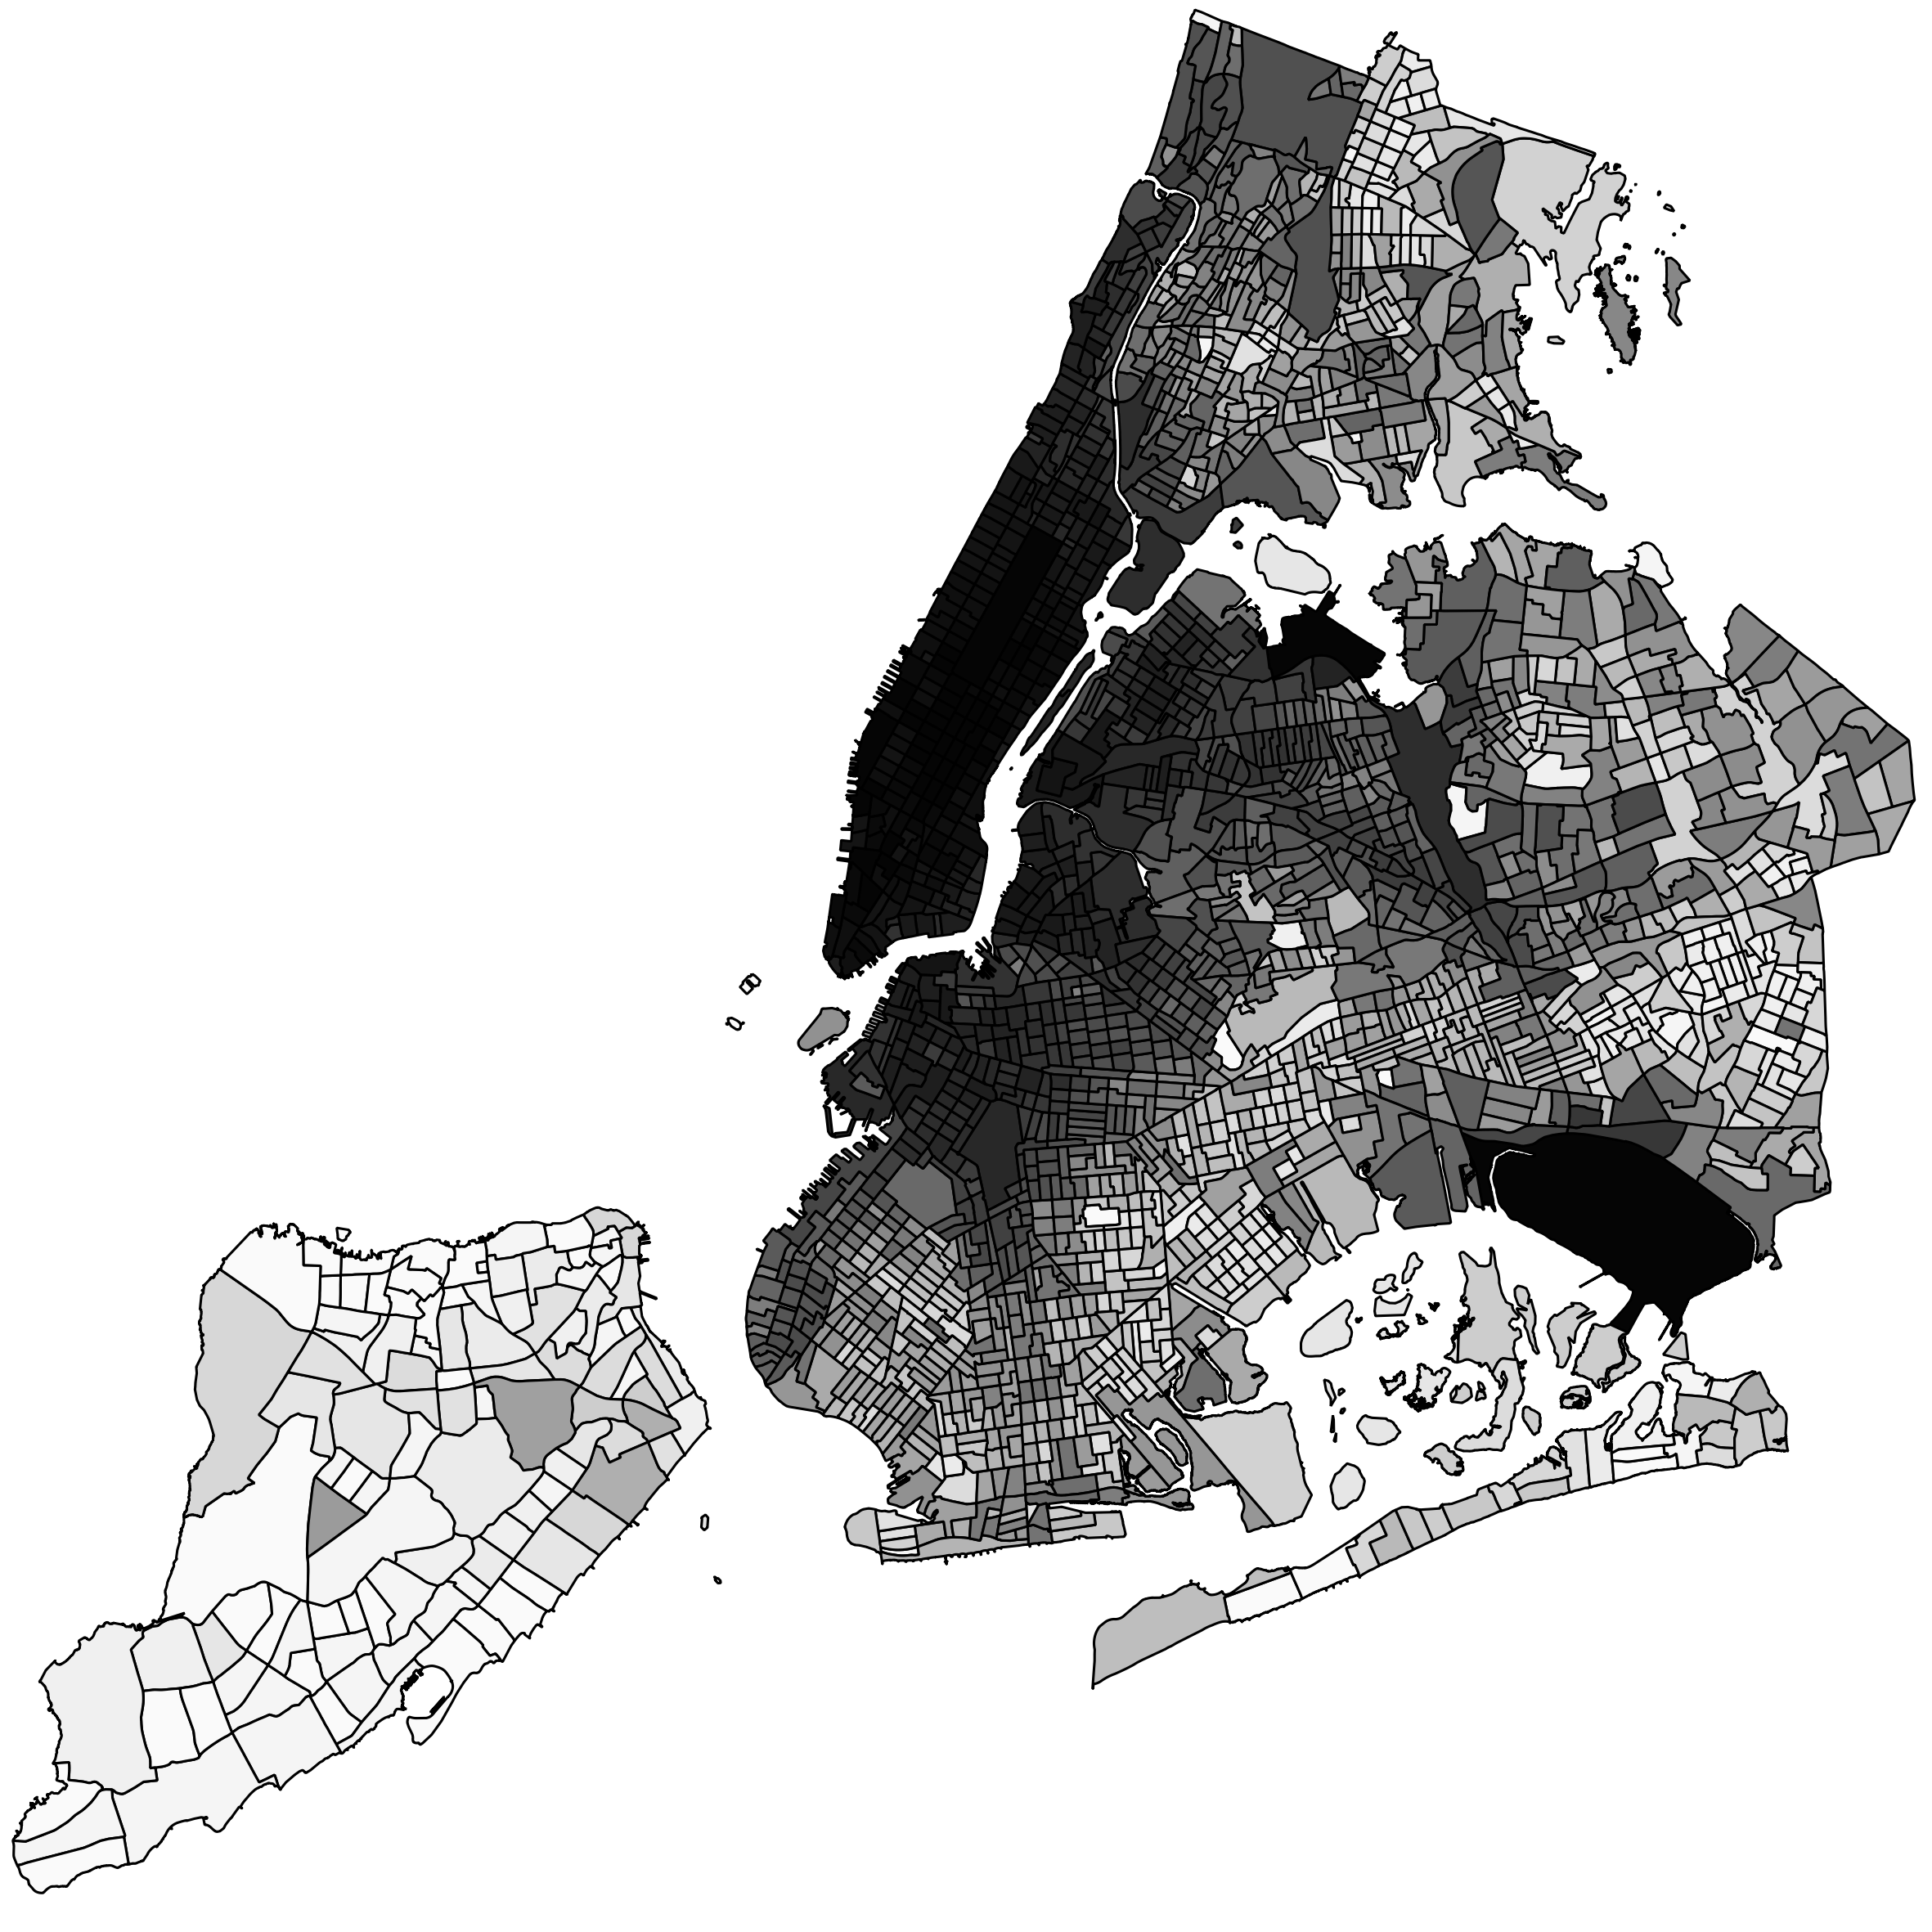
\includegraphics[scale=0.25, natwidth=2362, natheight=2362]{TotalDropoffsGreyscaletemp.png}
\end{centering}
% \caption{Map of New York City per-capita drop-offs. Staten Island is the island to the south-west with an overall low number of drop-offs, while Manhattan, where the chief central business district of the city is located, is the long, narrow island with a large number of drop-offs. \label{fig:map}}
%\end{figure}

%\todo{Really need to edit paragraph on the question actually answered to make it clearer.}

Note that I removed Staten Island, the island on the lower left of the map, from my analysis. Staten Island is extremely demographically and economically distinct from the rest of New York City, so much so that Staten Island actually voted in a referendum to secede from the city in 1993. 

By looking at the demographics of the locations where drop-offs occur, we can try to gain a bit of understanding of the demographic factors that effect ridership.
It's important to note though that not every drop-off represents someone getting dropped off at their home, so the location of drop-offs will not directly tell us who is taking taxis - far from it. This is clear if you look the few areas, such as central park and major transit hubs such as Penn Station and Grand Central which have drop-off rates orders of magnitude above the rest of the pack.
This large number of drop-offs does not come from residents, but from people from all over the city traveling to these popular destinations.
The mantra that correlation does not imply causation is probably worth repeating here, and it may be that a model based only on demographic factors is only useful as a first step to a more complete model rather that one where we should be making decisions right off the bat.
%We are finding what demographic factors are correlated with making a location popular for drop-offs, and it will probably take a lot more study to understand the causation between these demographic factors and drop-offs.
%We have to be careful not to confuse the effect of such destinations on demographics for direct effects of demographics on taxicab rides.

%The model I create based just on demographics may have  used as a first step to a better model
% As a result of the importance of factors that are not included in the demographics of residents, it may be that a model created based only on these demographics is more useful as a first step to a more complete model rather than one 
% It cannot be stressed enough though that this is not a direct measurement of these demographic factors.


%\todo{Paragraph explaining the map. Probably add a map of pc income}

%\todo{Paragraph explaining basics of analysis. Should include an equation, but that's the ONLY one.}

To do this analysis, I first studied correlations between the number of drop-offs and the various demographic features of each census tract in order to select out the demographic features which did the best job at predicting the number of drop-offs.
This indicated that the income of each census tract is highly correlated with the number of drop-offs, so I performed a regression to find how exactly income is related to drop-offs. The regression indicated that 
\begin{equation}
  \label{eq:PoissonFit}
  \mbox{\it per-capita drop-offs} \approx \frac{\left(\mbox{\it per-capita income}\right)^2}{4.7\times 10^8},
\end{equation}

When I say that the number of drop-offs per-capita is proportional to the square of the per-capita income, what this is really saying is something about the {\it average} number of drop-offs.
If we have a bunch of census tracts with the exact same per-capita income, we would not expect them all to have the exact same number of drop-offs per-capita.
Instead, the model says that they will all have different drop-offs per-capita, but their average will follow equation \ref{eq:PoissonFit}.
The model also gives a fairly specific description of how many tracts we'd expect to deviate from the average by how much, and this is where we start running into problems.

For the sake of comparison, lets imagine a New York where the probability of a taxicab dropping somebody off in a given census tract at any time depended on one thing, and one thing only - the per-capita income in that census tract.
In this imaginary world, if we looked at two census tracts with the exact same income, we wouldn't expect them to have the exact same number of drop-offs within a year, but we would expect them to be pretty close.
The thing is, if we look at two census tracts with similar per-capita incomes in the real data, the number of drop-offs is a whole lot less close than we'd expect if per-capita income was the only thing that mattered.

This means that there must be something other than per-capita income that matters here.
Frankly, that's not surprising - if I told you that per-capita income really was the {\it only} thing that mattered, it would be much more shocking.
The thing is that our data is {\it so} much farther apart than we'd expect if per-capita income was the only thing that mattered - about half a million times farther apart.
This means that there must be a whole lot more important factors that come in to play.

However, using just income does do a pretty good job of explaining things.
On a scale that goes from not explaining anything at all to explaining everything perfectly, using just income gets us about 65\% of the way to perfect - or for those who are familiar with regression, $R^2=0.65$\footnote{Technically this isn't an $R^2$ which doesn't really exist for Poisson regression. Instead, it is a ``$\mbox{pseudo-}R^2$'', which behaves a bit like an $R^2$ from ordinary least squares in that it represents the improvement over a null model. }.
That's a whole lot of the way to perfect using just a single variable.



Which other factors are important is still an open question.
A bunch of the possibilities are things that should be able to get data for such as the number of people who's place of work is in a given area, whether or not the residents commute in cars, or how far the area is from the city center.
But there also are plenty of factors that we can't hope to measure using a data driven approach, such as the presence of cultural institutions or a school dorm full of students who may be a whole lot wealthier than their income suggests.

Some of the factors that might be involved can't be seen by looking at the demographics of residents, like how many people's jobs are in a census tract.
And some of the factors are things that we can't expect to see directly, like the presence of cultural institutions.
However, many of the things that we may not be able to measure directly may have indirect effects on data that we can measure.
It could be that this is the reason that income is particularly useful, as factors like race, local employment, and cultural institutions are all correlated with income.
%Many of the things that will make people take cabs somewhere are the will also drive up real estate prices too.
%If residents want to be close to cultural institutions and their place of employment, areas that have this convenience will have higher real estate prices and attract wealthier residents, so per-capita income is capturing some of these effects was well.
%Thus, we would expect that the relationship between per-capita income and drop-offs might have a lower power if other factors were accounted for.

It is also important to not take .
I am looking at the  demographics of the locations where drop-offs occur,  not directly at the demographics of passengers, which could be dramatically different from data I'm measuring, especially if income is 






Based on this analysis, we can see that per-capita income is an impressive predictor for taxicab drop-offs, with a \prsq of 0.65.
However, the high dispersion parameter, along with the poor fit of the deviance residuals to a normal distribution indicates that the model may still have much room for improvement.
A possible avenue may be adding more demographic predictors, such as the average commute time, car usage, spatial position, or the racial make-up of census tracts. Borough, which may be a rough proxy for any of these possible predictors can be seen to correlate will with drop-offs in \fref{dropoffsvsincome}.
However, while there may be interesting information to be gleaned from exploring which predictors are the most successful, the room for improvement in this model largely lies in the distribution of the predicted error, and thus would probably be relatively marginal.

It is also possible that no improvement can be achieved from a demographic data based approach.
It may be that the effect from factors like transit hubs and cultural institutions that are particular to each individual census tract cannot be fully expressed through demographic data, and may not be able to be reasonably tracked by any data.

I, for one, find the simplicity of this model appealing: per-capita dropoffs are proportional to the square of per-capita income.
While there are clearly more details, the simple take away here is very satisfying.

%\todo{Write a lay-person readable blog post.}

%\todo{Write conclusion}
%\todo{Talk about boro as a possible predictor, but also mention others}



% - mostly. People with more income are also more likely to own a car themselves, and thus not need a taxicab in the first place. 
%Thus, if we look at just the census tracts where very few people commute by car, we find a nice, simple relationship between per-capita taxicab drop-offs (dropoffs) and per-capita income (income):
% $$
% \mathrm{dropoffs}\approx \frac{\mathrm{income}^{2.34}}{4.07\times 10^{10}}
% $$
% After discarding 10 high leverage points and outliers, this data set is pretty close to perfect for regression, with a fairly normal distribution of the data.
% The outliers consist of three major transportation hubs and two census tracts whose only residences are probably homeless shelters or college dorms, and are not surprising as outliers. The high-leverage (i.e. extreme income) points are all tracts on the Upper East Side next to central park, which I believe may be the highest income tracts in the nation.
% This fit is fairly strong, and with $R^2=0.71$, much of the variance is explained through regression.

% This data, however, only includes 672 of the 2083 census tracts with populations above 1000 (tracts with lower populations are largely parks and airports; there is no reason to think that taxicab drop-offs in these locations are representative of residents).
% The other 1411 data points with rates of car commuting above 20\% don't show a correlation with income, and it seems like they may be best explained with data that combines public transit usage with some measure of travel times to the central business district, though I am still working on finding the best data and the best way to combine them.




%\theendnotes



\newpage


\listoftodos
\end{document}


Because of smartphone apps like Uber, taxi politics has gotten a bunch of press lately. One of the claims that Uber proponents make is that normal taxis do not serve everybody.

In New York City, taxis are heavily regulated. There are only about 14,000 taxis allowed to pick up passengers off the street in the center of the city. Uber gets around this regulation by only picking up passengers who request a ride on the app.

Because there are few taxis, critics say that they can get away with only serving the few. Taxis only serve those with the privilege to live in the city center, the rich, and are biased against people of color. 

As a New Yorker who has spent my fair share of time waiting in taxi traffic on my bicicle, I wanted to get some understanding about the users of taxis in New York City. Are taxis actually unfair as critics claim? I looked at the locations where taxis drop off passengers. Then I looked to see if the locations correlate with demographic data about residents.

The drop off location data comes from the GPS in the taxi's meter. This data is recorded by the Taxi and Livery Cab Commission, which is nice enough to publish it on its website.

The demographic data comes from the United States Census Bureau.  They group NYC into about 2,000 regions that are usually just a few city blocks called census tracts. The data they gather includes race, age, commute mode, and income, among others.

Assigning a census tract to each GPS drop off point is no easy task. It's a computationally intensive job that I did using PostGIS. PostGIS has an efficient algorithm just for this job. But even with that, it would have taken too long for my laptop to match all 150 million drop offs.

Instead, I found the census tract of every point on a grid that divides the city into increments of one one-thousandth of a degree. Then, I could find the tract of a drop off GPS point just by rounding to the nearest one thousandth of a degree. This reduced the work the computer needed to do by a factor of ten.

A little note about the data: I removed Staten Island. For those not familiar with NYC geography, Staten Island is the island on the lower left of the map. It's much lighter than the rest of the city as it has few drop offs. It is economically, demographically, and culturally distinct from the rest of New York City. Even Staten Islanders agree: in 1993 they passed a referendum to secede from the city. The state of New York ignored them though. I respect the wishes of the residents and have seceded them from my analysis.

I found that the per capita income of residents is good at predicting the number of taxi drop offs. I did a Poisson regression and found that the number of drop offs per resident is proportional to the square of per capita income.

But it's important to keep in mind that drop offs do not necessarily represent residents. Something tells me that the 25 residents of Central Park didn't take 84,807 taxi rides each in 2013. There are many popular destinations within the city that attract people from everywhere. It seems like these same destinations may make rich people want to live there.

When I say that drop offs are proportional to the square of per capita income, this refers to the average that the model predicts. The model also expects that actual data will be randomly distributed around that average in a certain way. This is where a model based only on per capita income doesn't do so well. If per capita income were really the only thing that mattered, we would expect drop off data to be spread around the average by a certain amount. The actual data is spread about half a million times as much. Of course there is a lot more to the story than per capita income, but the large size of the extra spread implies that there is a whole lot more.

It's possible that I could improve the model by adding more demographic factors, but my initial analysis says that it won't make a significant improvement. It could be that a non-demographic factor would make a big improvement. I would imagine that looking at the number of employees who work in a census tract would improve the model. It also could be that there are too many significant factors that are immeasurable. Popular locations like Central Park and Penn Station may attract people at significant rates. Directly measuring the number of people that travel to an area every day isn't possible.

Using just income does do a pretty good job of explaining things. On a scale that goes from not explaining anything at all to explaining everything perfectly, it gets about 65% of the way to perfect.  For those who are familiar with regression, $R^2=0.65$.

I, for one, find the simplicity of this model appealing: per capita drop offs are proportional to the square of per capita income. While there are clearly more details, the simple take away here is quite satisfying.

Thomas Proctor has a brand new, shiny physics Ph.D.. His research simulates ferromagnets, like the magnets on your fridge, on a molecular-ish level. He hopes that in 20 years or so it will result magnets that are even stronger than the strongest we have now, but he's not about to bet on it. He spends his free time on his bicycle, both in his hometown of New York City, where it's his main source of transport, and in his travels around the world.


The map below shows New York City, divided up by census tract. Darker census tracts have a high number of drop offs, while lighter ones have less. 
